\documentclass{article}

\usepackage[margin=1in]{geometry}
\usepackage{graphicx} % Allow image/pdf includes
\usepackage{extramarks} % Extra header marks (continued on next page)
\usepackage{amsmath} % Math enhancements
\usepackage{amsthm} % Theorem typesetting
\usepackage{amssymb} % Extended symbol collection
\usepackage{tikz} % Graphical element creation
\usetikzlibrary{automata,positioning}
\usepackage{algpseudocode} % Algorithm layout
\usepackage{enumitem} % Enumerate (lists)
\usepackage{ragged2e} % Alternative alignment
\usepackage{gensymb} % Generic symbols (degree, etc)
\usepackage{empheq} % Allow \boxed around \begin{empheq}
\usepackage{color,soul} % Highlighting
\usepackage{booktabs} % Enhanced table creation
\usepackage{multirow} % Table multi row
\usepackage{mathtools} % Math enhancements
\usepackage{bm} % Bold math
\usepackage[mathscr]{euscript} % Script variables
\usepackage{cancel} % Cancel through text
\usepackage{color,soul} % Highlighting
\usepackage{mathtools}
\usepackage{multirow}
\usepackage{mathrsfs}
\usepackage{physics}
\usepackage{gensymb}
\usepackage{siunitx}
\usepackage{subcaption}
\usepackage[]{algorithm2e}
\usepackage{float}
\usepackage[cache=false]{minted}
\renewcommand{\MintedPygmentize}{/Users/loganharbour/miniconda/bin/pygmentize}
\usepackage[scaled]{beramono}
\usepackage[T1]{fontenc}

\setlength\parindent{0pt} % No indents
\setlength{\parskip}{1em} % Paragraph skip

\newcommand{\vx}{\mathbf{x}} % x vector
\newcommand{\vy}{\mathbf{y}} % x vector

\newcommand{\pageTitle}{MEEN 644 - Homework 3}
\newcommand{\pageAuthor}{Logan Harbour}

\begin{document}

\title{\LARGE \textbf{\pageTitle} \vspace{-0.3cm}}
\author{\large \pageAuthor}
\date{\vspace{-0.6cm} \large \today \vspace{-0.4cm}}

\maketitle

\section*{Problem statement}

Consider a thin copper square plate of dimensions 0.5 m $\times$ 0.5 m. The temperature of the west and south edges are maintained at 50 $^\circ$C and the north edge is maintained at 100 $^\circ$C. The east edge is insulated. Using finite volume method, write a program to predict the steady-state temperature solution.

\begin{enumerate}[label=(\alph*)]
	\item \textbf{(35 points)} Set the over relaxation factor $\alpha$ from 1.00 to 1.40 in steps of 0.05 to identify $\alpha_\text{opt}$. Plot the number of iterations required for convergence for each $\alpha$.
	\item \textbf{(15 points)} Solve the same problem using $21^2, 25^2, 31^2$, and $41^2$ CVs, respectively. Plot the temperature at the center of the plate (0.25 m, 0.25 m) vs CVs.
	\item \textbf{(10 points)} Plot the steady state temperature contour in the 2D domain with the $41^2$ CV solution.
\end{enumerate}

\section*{Preliminaries}

\subsection*{Two-dimensional heat conduction}

With two-dimensional heat conduction with constant material properties, insulation on the right and prescribed temperatures on all other sides, we have the PDE
\begin{equation}
	\begin{cases}
		k \pdv{^2T}{x^2} + k \pdv{^2T}{y^2} = 0\,,\\
		T(x, 0) = T_B\,,\\
		T(0, y) = T_L\,,\\
		T(0, L) = T_T\,,\\
		-k \pdv{T}{x} \Big|_{x = L} = 0\,,
	\end{cases}
\end{equation}
where
\begin{align*}
	T_B & \equiv 50~^\circ\text{C}\,, & T_L & \equiv 50~^\circ\text{C}\,, & T_T & \equiv 100~^\circ\text{C}\,.\\
	k & \equiv 386~\text{W/m}~^\circ\text{C}\,, & L & \equiv 0.5~\text{m}\,.\\
\end{align*}

We discretize the region on $x \times y = [0, L]^2$ by $N^2$ internal nodes with $\Delta x = x / N, \Delta y = y / N$.

\subsection*{Control volume equations}

Integrate over an internal control volume $(i,j)$ to obtain
\begin{align*}
	k \iint_{CV_{i, j}} \left[ \pdv{^2T}{x^2} + \pdv{^2T}{y^2} \right] dxdy & = 0\,, \quad (i, j) \in [2, 3, \ldots, N - 1]^2\,.\\
	k \Delta y \left[ \pdv{T}{x}\Big|_{w_{i,j}} - \pdv{T}{x}\Big|_{e_{i,j}} \right] + k \Delta x \left[ \pdv{T}{y}\Big|_{n_{i,j}} - \pdv{T}{y}\Big|_{s_{i,j}} \right] & = 0\,, \quad (i, j) \in [2, 3, \ldots, N - 1]^2\,.
\end{align*}
Now use the two node formulation for the derivative terms to obtain
\[
	k \Delta y \left[\frac{T_{E_{ij}} - T_{P_{ij}}}{\Delta x} - \frac{T_{P_{ij}} - T_{W_{ij}}}{\Delta x}\right] + k \Delta x \left[ \frac{T_{N_{ij}} - T_{P_{ij}}}{\Delta y} -\frac{T_{P_{ij}} - T_{S_{ij}}}{\Delta y} \right] = 0\,, \quad (i, j) \in [2, 3, \ldots, N - 1]^2\,.
\]
Collect like terms and modify the index to obtain
\begin{equation}
	\label{eq:internal}
	T_{i,j} a_p - T_{i, j+1} a_n - T_{i+1, j} a_e - T_{i, j-1} a_s - T_{i-1, j} a_w = 0\,,\quad (i, j) \in [2, 3, \ldots, N - 1]^2\,,
\end{equation}
where
\[
	a_n \equiv \frac{k \Delta y}{\Delta x}\,, \quad a_e \equiv \frac{k \Delta x}{\Delta y}\,, \quad a_s \equiv \frac{k\Delta y}{\Delta x}\,, \quad a_w \equiv \frac{k\Delta x}{\Delta y}\,, \quad a_p \equiv a_n + a_e + a_s + a_w\,.
\]

The remaining equations are solved similarly but with slight differences depending on which boundary the CV is on.

\subsection*{Solving method}

The problem is to be solved by the line-by-line method. In specific, the sweeping arrangement is: \textbf{south to north, west to east, north to south, east to west}. In this method, the contribution from one direction in a given control volume is lagged and moved to the right hand side in order to solve a tri-diagonal system. Convergence is declared when
\begin{equation}
	R = \sum_\text{CV} \left| a_p T_p - \sum_{\text{nb}} a_\text{nb} T_\text{nb} b_p\right|\leq 10^{-5}\,.
\end{equation}

Upon solving an individual system $Ax^{\ell + 1} = b$ with relaxation (where $\ell$ is the iteration index), the system is relaxed with the coefficient $\alpha$ by modifying it after construction by
\[
	\begin{cases}
		a_{ii} = a_{ii} / \alpha\,,\\
		b_i = b_i + (\alpha^{-1} - 1) a_{ii} x_i^\ell\,,
	\end{cases} \quad i = 1, \ldots, N\,,
\]
and it is then solved using the standard TDMA algorithm.

\section*{Results}

\subsection*{Part a}

With the given range of $\alpha$, it was determined for this specific problem with $15^2$ CVs that $\alpha_\text{opt} \approx 1.3$. The solve did not converge (with an attempted 1,000 iterations) for $\alpha = 1.4$. The requested figure showing the iteration need for each relaxation parameter follows in Figure \ref{fig:iterations}.

\begin{figure}[H]
	\centering
	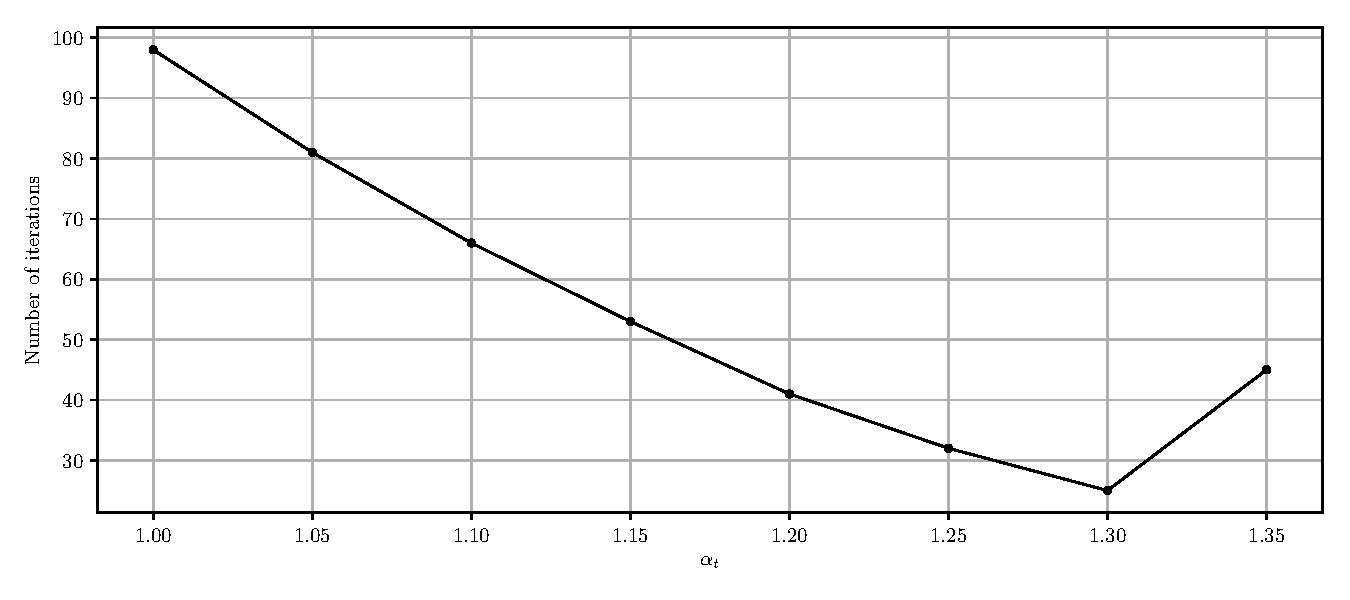
\includegraphics[width=\linewidth]{../python/iterations}
	\caption{Plot of the required iterations for each over relaxation factor.}
	\label{fig:iterations}
\end{figure}

\subsection*{Part b}

With a mesh refinement of $21^2, 25^2, 31^2,$ and $41^2$ CVs, the center temperature for each refinement is plotted below in Figure \ref{fig:center}.

\begin{figure}[H]
	\centering
	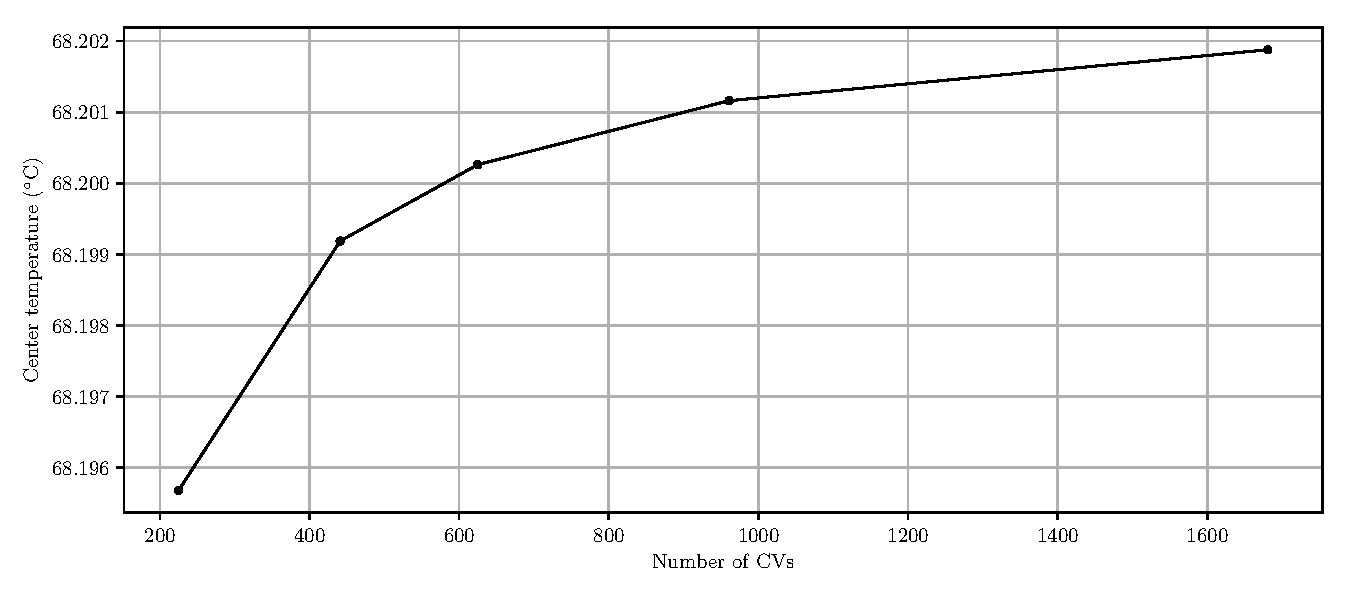
\includegraphics[width=\linewidth]{../python/center}
	\caption{Plot of the center temperature with mesh refinement.}
	\label{fig:center}
\end{figure}

\subsection*{Part c}

With the final mesh refinement of $41^2$ CVs, a colored contour plot of the temperature solution follows in Figure \ref{fig:solution}.

\begin{figure}[H]
	\centering
	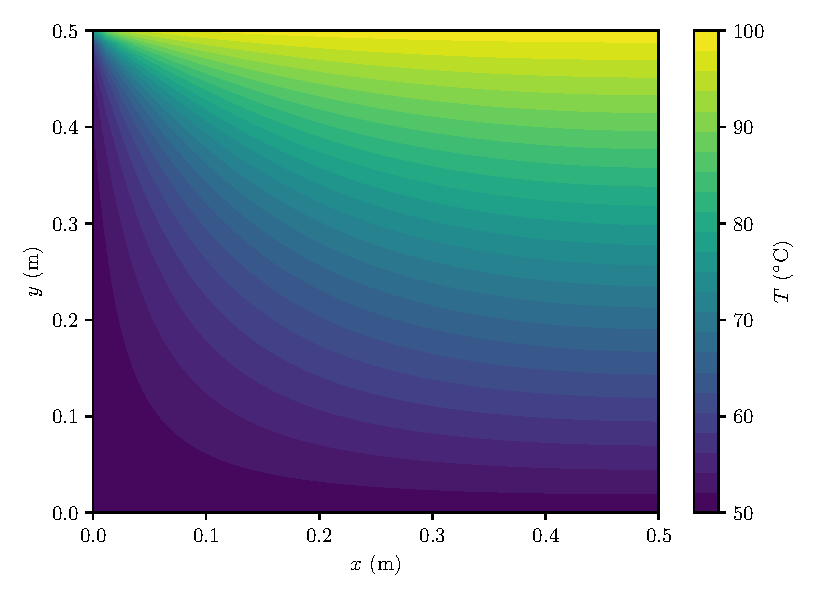
\includegraphics[width=0.7\linewidth]{../python/solution}
	\caption{Plot of the solution with $41^2$ CVs.}
	\label{fig:solution}
\end{figure}

\section*{Code listing}

\subsection*{Makefile}

\begin{minted}[fontsize=\small]{makefile}

src = $(wildcard *.cpp)
obj = $(src:.cpp=.o)
CXXFLAGS = -std=c++14
CCFLAGS = $(CXXFLAGS)

hwk-opt: $(obj)
	clang++ -o $@ $^

.PHONY: clean
	clean:
	rm -f $(obj) hwk-opt

\end{minted}

\subsection*{main.cpp}

\begin{minted}[fontsize=\small]{c++}

#include "Conduction2D.h"

int main() {
  // Part a: change relaxation factor
  std::cout << "Part a" << std::endl;
  for (double w : {1.0, 1.05, 1.10, 1.15, 1.20, 1.25, 1.30, 1.35, 1.40}) {
    std::cout << " Running with w = " << w << ": ";
    Conduction2D problem(15, 15, w);
    problem.solve();
  }
  std::cout << std::endl;

  // Part b: refine mesh and retreive center value
  std::cout << "Part b" << std::endl;
  for (unsigned int N : {15, 21, 25, 31, 41}) {
    std::cout << " Running with " << N * N << " CVs: ";

    Conduction2D problem(N, N, 1.3);
    problem.solve();
    std::cout << "  Center solution = " << std::setprecision(10)
              << problem.getT()((N - 1) / 2, (N - 1) / 2) << " C" << std::endl;

    // Part c: save finest solution
    if (N == 41)
      problem.save("solution.csv");
  }

  return 0;
}

\end{minted}

\subsection*{Conduction2D.h}

\begin{minted}[fontsize=\small]{c++}

#ifndef CONDUCTION2D_H
#define CONDUCTION2D_H

#include <iostream>
#include <iomanip>
#include <cmath>
#include <fstream>

#include "Matrix.h"
#include "TriDiagonal.h"

class Conduction2D {
public:
  Conduction2D(unsigned int Nx, unsigned int Ny, double alpha, double Lx = 0.5,
               double Ly = 0.5, double k = 386.0, double T_L = 50.0,
               double T_T = 100.0, double T_B = 50.0, double tol = 1e-5,
               unsigned int max_its = 1000);

  void solve();

  unsigned int getNx() { return Nx; }
  unsigned int getNy() { return Ny; }
  const Matrix & getT() const { return T; }
  void save(std::string filename) const { T.save(filename); }

private:
  double computeResidual() const;

  // Precompute operations
  void precomputeProperties();
  void precomputeColumn(unsigned int col);
  void precomputeRow(unsigned int row);

  // Solve and sweep operations
  void solveColumn(unsigned int col);
  void solveRow(unsigned int row);

protected:
  // Number of interior nodal points in the x and y-dimensions
  const unsigned int Nx, Ny;

  // Geometry [m]
  const double Lx, Ly, dx, dy;
  // Heat conduction coefficient [W / m k]
  const double k;
  // Dirichlet oundary conditions (left, top, bottom) [C]
  const double T_L, T_T, T_B;
  // Properties stored in matrix form
  Matrix a_p, a_n, a_e, a_s, a_w;

  // Inverse of the relaxation coefficient
  const double w_inv;
  // Iteration tolerance
  const double tol;
  // Maximum iterations
  const unsigned int max_its;

  // Temperature solution
  Matrix T;

  // Precomputed matrices for the TDMA solves
  std::vector<TriDiagonal> pre_A_x, pre_A_y;
  // Precomputed RHS for the TDMA solves
  std::vector<std::vector<double> > pre_b_x, pre_b_y;
  // Matrices for the TDMA solves
  TriDiagonal A_x, A_y;
  // RHS/solution vector for the TDMA solves
  std::vector<double> b_x, b_y;
};

#endif /* CONDUCTION2D_H */

\end{minted}

\subsection*{Conduction2D.cpp}

\begin{minted}[fontsize=\small]{c++}

#include "Conduction2D.h"

Conduction2D::Conduction2D(unsigned int Nx, unsigned int Ny, double w,
                           double Lx, double Ly, double k, double T_L,
                           double T_T, double T_B, double tol,
                           unsigned int max_its)
    : // Interior nodal points
      Nx(Nx), Ny(Ny), Lx(Lx), Ly(Ly), dx(Lx / Nx), dy(Ly / Ny),
      // Material properties
      k(k),
      // Boundary conditions
      T_L(T_L), T_T(T_T), T_B(T_B),
      // Material properties in matrix form
      a_p(Nx, Ny), a_n(Nx, Ny), a_e(Nx, Ny), a_s(Nx, Ny), a_w(Nx, Ny),
      // Solver properties
      w_inv(1.0 / w), tol(tol), max_its(max_its),
      // Initialize matrices and vectors
      T(Nx, Ny, (T_L + T_T + T_B) / 3.0), pre_A_x(Ny, Nx), pre_A_y(Ny, Nx),
      pre_b_x(Ny, std::vector<double>(Nx)),
      pre_b_y(Nx, std::vector<double>(Ny)), A_x(Nx), A_y(Ny), b_x(Nx), b_y(Ny) {
}

void Conduction2D::solve() {
  // Compute the a coefficients for each CV
  precomputeProperties();
  // Compute the unchanging LHS and RHS for each column
  for (unsigned int i = 0; i < Nx; ++i)
    precomputeColumn(i);
  // Compute the unchanging LHS and RHS for each row
  for (unsigned int j = 0; j < Ny; ++j)
    precomputeRow(j);

  // Iterate and exit when complete
  for (unsigned int l = 1; l <= max_its; ++l) {
    // Sweep south to north
    for (int j = 0; j < Ny; ++j)
      solveRow(j);
    // Sweep west to east
    for (int i = 0; i < Nx; ++i)
      solveColumn(i);
    // Sweep north to south
    for (int j = Ny - 1; j >= 0; --j)
      solveRow(j);
    // Sweep east to west
    for (int i = Nx - 1; i >= 0; --i)
      solveColumn(i);

    // Check for convergence
    double R = computeResidual();
    if (R < tol) {
      std::cout << "Converged with " << l << " iterations" << std::endl;
      return;
    }
  }

  std::cout << "Failed to converge in " << max_its << " iterations"
            << std::endl;
}

void Conduction2D::precomputeProperties() {
  // Set all neighbors to the default at first
  a_n = k * dx / dy;
  a_e = k * dy / dx;
  a_s = k * dx / dy;
  a_w = k * dy / dx;

  // Top Dirichlet
  a_n.setRow(Ny - 1, 2 * k * dx / dy);
  // Right Neumann
  a_e.setColumn(Nx - 1, 0);
  // Bottom Dirichlet
  a_s.setRow(0, 2 * k * dx / dy);
  // Left dirichlet
  a_w.setColumn(0, 2 * k * dy / dx);

  // Center point
  for (unsigned int i = 0; i < Nx; ++i)
    for (unsigned int j = 0; j < Ny; ++j)
      a_p(i, j) = a_n(i, j) + a_e(i, j) + a_s(i, j) + a_w(i, j);
}

void Conduction2D::precomputeRow(unsigned int j) {
  TriDiagonal &A = pre_A_x[j];
  std::vector<double> &b = pre_b_x[j];

  // First treat all as an internal volume
  A.addTopRow(a_p(0, j) * w_inv, -a_e(0, j));
  A.addBottomRow(-a_w(Nx - 1, j), a_p(Nx - 1, j) * w_inv);
  for (unsigned int i = 1; i < Nx - 1; ++i)
    A.addMiddleRow(i, -a_w(i, j), a_p(i, j) * w_inv, -a_e(i, j));

  // Left Dirichlet
  b[0] += T_L * a_w(0, j);
  // Top dirichlet
  if (j == Ny - 1)
    for (unsigned int i = 0; i < Nx; ++i)
      b[i] += T_T * a_n(i, j);
  // Bottom dirichlet
  else if (j == 0)
    for (unsigned int i = 0; i < Nx; ++i)
      b[i] += T_B * a_s(i, j);
}

void Conduction2D::precomputeColumn(unsigned int i) {
  TriDiagonal &A = pre_A_y[i];
  std::vector<double> &b = pre_b_y[i];

  // First treat all as an internal volume
  A.addTopRow(a_p(i, 0) * w_inv, -a_n(i, 0));
  A.addBottomRow(-a_s(i, Ny - 1), a_p(i, Ny - 1) * w_inv);
  for (unsigned int j = 1; j < Ny - 1; ++j)
    A.addMiddleRow(j, -a_s(i, j), a_p(i, j) * w_inv, -a_n(i, j));

  // Left Dirichlet
  if (i == 0)
    for (unsigned int j = 0; j < Ny; ++j)
      b[j] += T_L * a_w(i, j);
  // Top Dirichlet
  b[Ny - 1] += T_T * a_n(i, Ny - 1);
  // Bottom Dirichlet
  b[0] += T_B * a_s(i, 0);
}

void Conduction2D::solveRow(unsigned int j) {
  // Copy pre-filled Ax = b for this row
  A_x = pre_A_x[j];
  b_x = pre_b_x[j];

  // RHS contribution from volumes above and below
  if (j > 0)
    for (unsigned int i = 0; i < Nx; ++i)
      b_x[i] += T(i, j - 1) * a_s(i, j);
  if (j < Ny - 1)
    for (unsigned int i = 0; i < Nx; ++i)
      b_x[i] += T(i, j + 1) * a_n(i, j);

  // Relax, solve, and store solution (which is in b_x)
  if (w_inv != 1)
    for (unsigned int i = 0; i < Nx; ++i)
      b_x[i] += (w_inv - 1.0) * a_p(i, j) * T(i, j);
  A_x.solveTDMA(b_x);
  T.setRow(j, b_x);
}

void Conduction2D::solveColumn(unsigned int i) {
  // Copy pre-filled Ax = b for this row
  A_y = pre_A_y[i];
  b_y = pre_b_y[i];

  // RHS contribution from volumes left and right
  if (i > 0)
    for (unsigned int j = 0; j < Ny; ++j)
      b_y[j] += T(i - 1, j) * a_w(i, j);
  if (i < Nx - 1)
    for (unsigned int j = 0; j < Ny; ++j)
      b_y[j] += T(i + 1, j) * a_e(i, j);

  // Relax, solve, and store solution (which is in b_y)
  if (w_inv != 1)
    for (unsigned int j = 0; j < Ny; ++j)
      b_y[j] += (w_inv - 1.0) * a_p(i, j) * T(i, j);
  A_y.solveTDMA(b_y);
  T.setColumn(i, b_y);
}

double Conduction2D::computeResidual() const {
  double R = 0.0, val = 0.0;
  // Sum over all CVs
  for (unsigned int i = 0; i < Nx; ++i)
    for (unsigned int j = 0; j < Ny; ++j) {
      // Main diagonal contribution and pre-computed RHS (from BC)
      val = a_p(i, j) * T(i, j) - pre_b_y[i][j];
      // Not on left boundary
      if (i > 0)
        val -= a_w(i, j) * T(i - 1, j);
      // Not on right boundary
      if (i < Nx - 1)
        val -= a_e(i, j) * T(i + 1, j);
      // Not on bottom boundary
      if (j > 0)
        val -= a_s(i, j) * T(i, j - 1);
      // Not top boundary
      if (j < Ny - 1)
        val -= a_n(i, j) * T(i, j + 1);
      R += std::abs(val);
    }
  return R;
}

\end{minted}

\subsection*{Matrix.h}

\begin{minted}[fontsize=\small]{c++}

#ifndef MATRIX
#define MATRIX

#define NDEBUG
#include <cassert>

#include <vector>

class Matrix {
public:
  Matrix(unsigned int Nx, unsigned int Ny, double v = 0)
      : Nx(Nx), Ny(Ny), M(Nx, std::vector<double>(Ny, v)) {}

  // Const operator for getting the (i, j) element
  const double &operator()(unsigned int i, unsigned int j) const {
    assert(i < Nx && j < Ny);
    return M[i][j];
  }
  // Operator for getting the (i, j) element
  double &operator()(unsigned int i, unsigned int j) {
    assert(i < Nx && j < Ny);
    return M[i][j];
  }
  // Operator for setting the entire matrix to a value
  void operator=(double v) {
    for (unsigned int j = 0; j < Ny; ++j)
      setRow(j, v);
  }

  // Saves the matrix in csv format
  void save(const std::string filename, unsigned int precision = 12) const {
    std::ofstream f;
    f.open(filename);
    for (unsigned int j = 0; j < Ny; ++j) {
      for (unsigned int i = 0; i < Nx; ++i) {
        if (i > 0)
          f << ",";
        f << std::setprecision(precision) << M[i][j];
      }
      f << std::endl;
    }
    f.close();
  }

  // Set the j-th row to v
  void setRow(unsigned int j, double v) {
    assert(j < Ny);
    for (unsigned int i = 0; i < Nx; ++i)
      M[i][j] = v;
  }
  // Set the i-th column to v
  void setColumn(unsigned int i, double v) {
    assert(i < Nx);
    for (unsigned int j = 0; j < Ny; ++j)
      M[i][j] = v;
  }

  // Set the j-th row to vs
  void setRow(unsigned int j, std::vector<double> &vs) {
    assert(j < Ny && vs.size() == Nx);
    for (unsigned int i = 0; i < Nx; ++i)
      M[i][j] = vs[i];
  }
  // Set the i-th column to vs
  void setColumn(unsigned int i, std::vector<double> &vs) {
    assert(i < Nx && vs.size() == Ny);
    for (unsigned int j = 0; j < Ny; ++j)
      M[i][j] = vs[j];
  }

private:
  // The size of this matrix
  const unsigned int Nx, Ny;

  // Matrix storage
  std::vector<std::vector<double> > M;
};

#endif /* MATRIX_H */

\end{minted}

\subsection*{TriDiagonal.h}

\begin{minted}[fontsize=\small]{c++}

#ifndef TRIDIAGONAL_H
#define TRIDIAGONAL_H

#define NDEBUG
#include <cassert>

/**
 * Class that holds a tri-diagonal matrix and is able to perform TDMA in place
 * with a given RHS.
 */
class TriDiagonal {
public:
  TriDiagonal(unsigned int N, double v = 0)
      : N(N), A(N, v), B(N, v), C(N - 1, v) {}

  // Operator for setting the entire matrix to a value
  void operator=(TriDiagonal & from) {
    assert(from.getN() == N);
    A = from.getA();
    B = from.getB();
    C = from.getC();
  }

  // Gets the value of the (i, j) entry
  const double operator()(unsigned int i, unsigned int j) const {
    assert(i < N && j > i - 2 && j < i + 2);
    if (j == i - 1)
      return A[i];
    else if (j == i)
      return B[i];
    else if (j == i + 1)
      return C[i];
    else {
      std::cerr << "( " << i << "," << j << ") out of TriDiagonal system";
      std::terminate();
    }
  }

  // Adders for the top, middle, and bottom rows
  void addTopRow(double b, double c) {
    B[0] += b;
    C[0] += c;
  }
  void addMiddleRow(unsigned int i, double a, double b, double c) {
    assert(i < N - 1 && i != 0);
    A[i] += a;
    B[i] += b;
    C[i] += c;
  }
  void addBottomRow(double a, double b) {
    A[N - 1] += a;
    B[N - 1] += b;
  }

  // Getters for the raw vectors
  const std::vector<double> &getA() const { return A; }
  const std::vector<double> &getB() const { return B; }
  const std::vector<double> &getC() const { return C; }

  // Getter for the size
  unsigned int getN() { return N; }

  // Solves the system Ax = d in place where d eventually stores the solution
  void solveTDMA(std::vector<double> &d) {
    // Forward sweep
    double tmp = 0;
    for (unsigned int i = 1; i < N; ++i) {
      tmp = A[i] / B[i - 1];
      B[i] -= tmp * C[i - 1];
      d[i] -= tmp * d[i - 1];
    }

    // Backward sweep
    d[N - 1] /= B[N - 1];
    for (unsigned int i = N - 2; i != std::numeric_limits<unsigned int>::max();
         --i) {
      d[i] -= C[i] * d[i + 1];
      d[i] /= B[i];
    }
  }

protected:
  // Matrix size (N x N)
  unsigned int N;

  // Left/main/right diagonal storage
  std::vector<double> A, B, C;
};

#endif /* TRIDIAGONAL_H */

\end{minted}


\end{document}
